\documentclass{article}
\usepackage{listings}
\usepackage{xcolor} % xcolor for HTML colors
\usepackage{dirtytalk}

\usepackage{graphicx}
\graphicspath{{./pages/diag/}}

% Night Owl Light
\definecolor{foreground}{HTML}{403f53}
\definecolor{background}{HTML}{FBFBFB}
\definecolor{comment}{HTML}{989fb1}
\definecolor{number}{HTML}{aa0982}
\definecolor{keyword}{HTML}{994cc3}
\definecolor{string}{HTML}{c96765}

\lstdefinestyle{haskell}{
    backgroundcolor=\color{background},   
    commentstyle=\color{comment},
    keywordstyle=\color{keyword},
    numberstyle=\small\color{black},
    stringstyle=\color{string},
    basicstyle=\ttfamily\small\color{foreground},
    breakatwhitespace=false,
    breaklines=true,
    captionpos=b,
    keepspaces=true,
    numbers=left,
    numbersep=5pt,
    showspaces=false,
    showstringspaces=false,
    showtabs=true,
    tabsize=2
}

\title{Haskell Study Notes}
\author{Charlotte}

% it's the only language we care about anyway 
\lstset{style=haskell}
\lstset{language=Haskell}

\begin{document}
\maketitle
\tableofcontents
\pagenumbering{arabic}

% Types
\section{Types}
\subsection{Basic types}
Haskell has many primitive types such as strings, characters, integers and floating point numbers.

\begin{lstlisting}
"hello world" -- string
1234          -- integer
3.14          -- float
\end{lstlisting}

\subsection{Typeclasses}
Typeclasses are a way of sharing specific functionality between types. We can either implement our
own instances of typeclasses, or let haskell \emph{derive} them automatically.

They are kind of like Java interfaces.

Num is the generic base typeclass that all numbers derive from.
\begin{enumerate}
    \item Integral numbers (\emph{Integral} typeclass)
    \begin{itemize}
        \item \emph{Int}: fixed precision integer with a min and maximum size
        \item \emph{Integer}: supports \textbf{very} large integers
    \end{itemize}
    \item Floating point numbers (\emph{Fractional} typeclass)
    \begin {itemize}
        \item \emph{Float}: single precision floating point number
        \item \emph{Double}: double precision floating point number
    \end{itemize}
\end{enumerate}

\subsection{More on typeclasses}
Anything that derives from
\begin{itemize}
    \item \emph{Show} can be printed
    \item \emph{Read} can be read as a value
    \item \emph{Eq} can be compared for equality with \emph{==} and \emph{/=}
    \item \emph{Ord} can be compared and ordered with \emph{<} and \emph{>}
\end{itemize}

\newpage
\begin{lstlisting}
{-# LANGUAGE DuplicateRecordFields #-}

data Worker = Worker { name :: String, job :: String } deriving (Show)
data Student = Student { name :: String, school :: String } deriving (Show)

class Person a where
    getName :: a -> String
    getOccupation :: a -> String

instance Person Worker where
    getName x = name (x :: Worker)
    getOccupation x = "Working on " ++ job x

instance Person Student where
    getName x = name (x :: Student)
    getOccupation x = "Studying at " ++ school x
\end{lstlisting}
\figurename{ 1: Demonstration of a custom typeclass for Person}
\section{Lists and Tuples}

\subsection{Lists}
Lists have a \emph{head} and a \emph{tail}. Because of Haskell being lazily evaluated, lists can be infinite.
\emph{take} takes \emph{n} items from a list, and \emph{drop} drops \emph{n} items from a list.\\
\\
list = [1, 2, 3, 4, 5]\\
In the above list, the \emph{head} is \underline{1}, and the \emph{tail} is \underline{[2, 3, 4, 5]}

\begin{lstlisting}
list = [1, 2, 3, 4, 5]
head list -- 1
tail list -- [2, 3, 4, 5]

-- take 10 elements from an infinite list
take 10 [1..]

-- if you try to just get the entire list, it will hang GHCI
-- since it will never end because the list is infinite in size
[1..]
\end{lstlisting}

Lists can be indexed using the \emph{!!} operator. 
\begin{lstlisting}
firstItem = list !! 0 -- lists start from 0    
\end{lstlisting}

\subsection{Tuples}
Haskell has tuples, triples, and \emph{n-tuples}. Tuples have a \emph{fst} and \emph{snd} function which
respectively gets either the first \underline{or} second item. 

\emph{swap} (defined in \textbf{Data.Tuple}) swaps the items in a \emph{tuple}

\begin{lstlisting}
("char", 20)

-- a triple
("char", 20, "turtles")
\end{lstlisting}
\section{Conditionals}
\subsection{If expressions}
Haskell doesnt have if statements, however it has if expressions instead.

\begin{lstlisting}
-- stolen from the haskell book
let x = 0
if (x + 1 == 1) then "AWESOME" else "wut"
\end{lstlisting}

\subsection{Case expressions}
Case expressions are similar to switch-case from languages like Java, and C++. Case expressions begin with \texttt{case x of} and their body contains all the different
cases in the format \emph{value} $\rightarrow$ \emph{return-value}.

\begin{lstlisting}
pal xs =
  case y of
    True  -> "yes"
    False -> "no"
  where y = xs == reverse xs
\end{lstlisting}

It can also be used to \emph{pattern match} against data types
\begin{lstlisting}
data Animal = Cat | Dog
speak a =
  case a of
    Cat -> "meow"
    Dog -> "bork"
\end{lstlisting}

\newpage
\subsection{Guards}
There are also guards which can provide a nicer way of pattern matching instead of writing if-else expressions or case blocks. Guard blocks are written as a series of
cases, along with a fallback case called \texttt{otherwise}

Cases are written in the format:
\say{$\vert$ \emph{condition} = \emph{value}.}

\begin{lstlisting}
abs n
  | n < 0     = -n
  | otherwise = n
\end{lstlisting}


\subsection{Pattern matching}
Pattern matching is very common in Haskell. It allows great flexibility since you can pattern match against anything to extract values etc.

\emph{\_} or \emph{x} means a catch-all/fallback pattern to match on if all else fails

\begin{lstlisting}
isItOne :: Int -> Bool
isItOne 1 = True
isItOne _ = False
\end{lstlisting}

\subsubsection{Matching against data constructors}
Pattern matching against data constructors is possible. The example defines two functions called \texttt{getName} and \texttt{getAccNumber} that
pattern match on the \emph{User} data constructor to extract either the name \underline{or} account number.

\begin{lstlisting}
data User = User String Int

getName :: User -> String
getName (User name _) = name

getAccNumber :: User -> Int
getAccNumber (User _ acc) = acc
\end{lstlisting}

\footnote{If we don't use a field, we can use an \_ just like pattern matching with functions to signify the field is ignored}
\footnote{
    Pattern matching against data constructors can get real old if you have a lot of parameters.
    So an alternative to this that will be covered later is record types.
}
\section{Functions}
Functions are defined like add x y = x + y. All functions are pure, unless stated otherwise which means
they cannot modify state, or perform \underline{side effects} like input output, writing to a database, etc

\subsection{Currying}
By default, all functions are curried in Haskell. Given the following type signature

\begin{lstlisting}
-- add takes two ints and returns an int
add :: Int -> Int -> Int
\end{lstlisting}

we would say that the function \textbf{add} takes two integers, and returns an integer.
However, because of how currying works it actually means.

\begin{itemize}
    \item \textbf{add} takes a \emph{single} integer parameter
    \item and returns a function that takes another integer parameter, and eventually
    will return an integer itself.
\end{itemize}

Currying is useful because it means we can create new functions by \emph{partially applying}
functions to parameters.

\begin{lstlisting}
-- desugared form of the above add function
add :: Int -> (Int -> Int)

addOne :: Int -> Int
addOne x = add 1

-- addOne 5 desugars to
addOne 5
((add 1) 5)
6
\end{lstlisting}

\subsection{Higher-order functions}
Higher order functions are functions that can accept functions as parameters
\emph{flip} is an example of a higher-order function.

Its type signature is \emph{flip :: (a $\rightarrow$ b $\rightarrow$ c) $\rightarrow$ b $\rightarrow$ a $\rightarrow$ c}
and it can be partially applied like so

\begin{lstlisting}
flipOne = flip 1
partialApply = flipOne 2 -- ((flip 1) 2)
\end{lstlisting}

\subsection{Function composition}
Composing functions is like a \emph{right to left} pipeline. \textbf{f . g} can be read
as \textbf{f} after \textbf{g}.

(f $\circ$ g) x = f (g x)
\begin{enumerate}
    \item first applies \emph{g}
    \item then applies \emph{f} to the result of applying \emph{g}
    \item and makes a new function which takes a parameter \emph{x}
\end{enumerate} 

Example of function composition in action
\begin{lstlisting}
negate . sum $ [1,2,3,4,5]

-- which is equivalent to
negate (sum [1,2,3,4,5])
negate (15)
\end{lstlisting}

\footnote{
    \$ is used since function application has the highest precedence, so Haskell will think we mean negate . 15.
    Alternatively, you can wrap it in brackets like \textbf{negate . (sum [1,2,3,4,5])}}
\section{Recursion}

\subsection{Factorial}
A classic way of demonstrating recursion is factorial. 4! means
4 * 3 * 2 * 1.

The broken down steps can be seen below.

\begin{verbatim}
4! = 4 * 3 * 2 * 1
       12  * 2 * 1
            24 * 1
               24
4! = 24
\end{verbatim}

The \emph{factorial} function can be defined in Haskell.
If there is no base case defined, the recursion will go on forever and will never stop.

\begin{lstlisting}
fac :: Integer -> Integer
fac 0 = 1 -- base case
fac n = n * fac (n -1)
\end{lstlisting}

\footnote{\emph{fac 0 = 1} is the base case since it will return 1, and stop the recursion.}

\subsection{More examples of recursion}
Some more examples of recursion from \emph{work/recursion.hs}.

\lstinputlisting[breaklines]{work/recursion.hs}

\newpage
\subsection{Foldl vs foldr style recursion}
\emph{foldr} folds a list from right to left, whereas \emph{foldl} folds
a list from left to right.

\emph{foldl} stacks parentheses on the left where as \emph{foldr} stacks them on the right
(((0+1)+2)+3) vs (1+(2+(3+0)))

\begin{figure}[h]
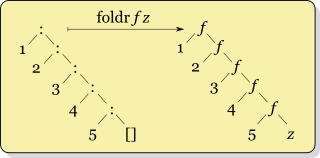
\includegraphics[width=0.7\textwidth]{foldr-rec.png}
\centering
\caption{foldr recursion}
\end{figure}

\begin{figure}[h]
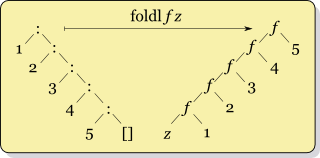
\includegraphics[width=0.7\textwidth]{foldl-rec.png}
\centering
\caption{foldl recursion}
\end
{figure}
\section{Weak head normal form}

Values in Haskell are reduced to Weak head normal form (WHNF).
Weak head normal form is a type of normal form which contains both the possibility the expression has been fully evaluated/reduced (normal form) as well as the possibility that the expression has been evaluated to the point of arriving at a data constructor/lambda waiting for an argument.

These expressions \textbf{are} in WHNF:

\begin{lstlisting}[linewidth=15cm]
-- https://stackoverflow.com/questions/6872898/
(1, 1 + 1)          -- outermost part is the data constructor (,)
\x -> 2 + 2         -- outermost part is a lambda abstraction
'h' : ("e" + "llo") -- outermost part is the data constructor (:)
\end{lstlisting}

These examples \textbf{are not} in WHNF
\begin{lstlisting}[linewidth=15cm]
1 + 2               -- the outermost part here is an application of (+)
(\x -> x + 1) 2     -- the outermost part is an application of (\x -> x + 1)
"he" ++ "llo"       -- the outermost part is an application of (++)    
\end{lstlisting}

We can use \texttt{:sprint} in GHCI to print out the representation of the value in memory. Due to laziness, polymorphic types are unevaluated (thunked) until we use them. This is marked with an underscore (\_).

\begin{verbatim}
Prelude> let nums = [1..5]

Prelude> :sprint nums
nums = _

Prelude> take 2 nums
Prelude> :sprint nums
nums = 1 : 2 : _
\end{verbatim}

\footnote{The examples on WHNF were taken directly from the amazing Haskell Book}

\end{document}